\documentclass{article}


%% Bring the margins down to 1 inch, like the old ``fullpage'' package.
\usepackage[margin=1.0in]{geometry}

\usepackage{graphicx}
\usepackage{caption}
\usepackage{subcaption}


%% Gives the equivalent of one-and-a-half line spacing.
\linespread{1.3}

\begin{document}

\section{Shanes's original bacteria data}

\subsection{Overview}

Our earlier work determined that analyses at the phylum-level did not
explain nearly as much of the variability as did models built on
family-level and order-level taxa.  So, we focused on the family and
order levels.  These taxa were obtained from 6 cadavers on 16 different
days.  However, taxa counts are not available for\\
- subject A1 on days 7 and 9\\
- subject A4 on day 7


Since our last meeting, I realized that the data collected from
subject A3 on day 40 (degree day 1130) appears to be defective.  The
total number of taxa (including unclassified taxa) counted for this
cadaver and day was 54.  This is several orders of magnitude less than
the counts for the other cadavers and days, which ranged from 18050 to
93665 (both orders and families).  For this reason, the taxa from
subject A3 on day 40 were omitted from all the analyses.  The omission
of the A3, day 40 data does not affect the analyses which only
consider the first two weeks or data.

For the analyses which considered all time steps, we have 92
observations (16 days $\times$ 6 cadavers, minus the 4 missing
cadaver-day combinations mentioned in the previous paragraphs).  For
the analyses considering the first 15 days (approximately two weeks),
we have 57 observations (10 days $\times$ 6 cadavers, minus the 3
missing cadaver-day combinations occurring during this period).


\subsection{Cross-validation procedures}

As a reminder, we use cross-validation to help us choose certain
settings for the random forest model.  The main parameter to optimize
is the number of variables which the model can consider at each
branching of the decision tree.  In my code, I call this value
\texttt{numVarSplit}.  A secondary parameter is the number of bootstrap
samples to use to build the random forest, but I found that about 300
samples seems to be sufficient for all the cases we've considered.

To estimate the \texttt{numVarSplit}, I used cross-validation
runs.  For each run, I randomly select a certain subset (a minority)
of the available observations to hold back as a ``validation'' data
set.  The rest of the observations make up the ``training'' dataset.
We then fit a series of random forest models on the training dataset,
using a variety of possible values for \texttt{numVarSplit}.  We then
use the models to predict the values for the validation dataset, and
calculate the errors (actual number of degree days from the validation
dataset minus the number of degree days estimated by the model).  The
setting for \texttt{numVarSplit} which produces the smallest error and
the greated fraction of variability explained is the one I use for the
final model.

I had some concerns about how well our model would perform in
prediction mode.  We have only 6 cadavers, and we only have
observations at certain time steps.  Since our last conversation, I've
reduced the training set to 80\% of the data, reserving 20\% to use as
a test set.  (Previously, the split was 90\% and 10\%.)  When using
all the data, this means training on a set of 74 observations, and
testing on a size of 18.  When using just the first 15 days of data,
this means training on a set of 46 observations, and testing on a size
of 11.  The change from 90\% to 80\% made very little difference in
the choice of models, which relieved some of my concern.

Since our last meeting, I figured out how to parallelize some of the
computational work, which allowed me to use some additional
cross-validation runs and to try additional models, compared to what I
had done previously.



\subsection{All time steps}

In this section, we utilize data collected on all available days.  The
number of days post mortem, along with the corresponding accumulated
degree days, are shown below.

\begin{center}
\begin{tabular}{r|rrrrrrrrrrrrrrrr}
  Day & 0 & 1 & 2 & 3 & 5 & 7 & 9 & 11 & 13 & 15 & 26 & 33 & 40 & 47 & 54 & 61\\
  Degree day & 0 & 27 & 57 & 87 & 149 & 209 & 267 & 326 & 390 & 448 & 734 & 930 & 1130 & 1326 & 1516 & 1703
\end{tabular}
\end{center}



\subsubsection{Results for family-level taxa}

In our original analysis, we excluded from the model any taxa which
made up less than 1\% of the observed taxa for all cadavers and all
days.  That is, in order to be included, a particular family-level
taxa had to make up at least 1\% of the counts on just one day for
just one individual.  This has the advantage of being an easy cutoff
to implement and to explain.  However, this means that a taxa can be
included based on one unusual observation, even if this taxa is rarely
observed in the vast majority of cases.

To address these concerns, I also ran the analyses with a stricter
cutoff criterion.  Now, in order to be considered in the random forest
model, a taxa must make up more at least 1\% of the counts for at
least two separate cadavers.  These exceedances can happen on the same
day or on different days.  This addresses the concern that one
particularly unusual cadaver can cause taxa to be considered in the
model which are not generally present on other cadavers.  It also
makes explaining the model a bit easier, because there are fewer taxa
to consider and outlying taxa are less likely to affect the fit.

To illustrate the differences, consider the analysis using
family-level taxa for all time steps.  Using the original cutoff
criterion, the model considers 49 possible family-level taxa.  The top
ten most influential taxa identified by the resulting model are shown
in Figure \ref{fig:infl_family_taxa_orig_crit}.  Their influence on the
model is determined by how much the node impurity (i.e., the
variability in the ``leaves'' of the decision tree) is reduced by
including these particular family-level taxa in the random forest
model.  That is, a more influential taxa is associated with a large
decrease in this variability.

\begin{figure}
  \centering
  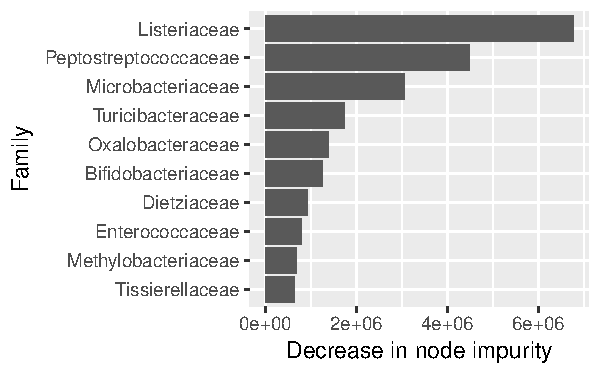
\includegraphics{../../only_families/all_time_steps/cutoff_1perc/orig_units_all_data_families_barchart}
  \caption{Ten most influential family-level taxa, modeled using a weak inclusion criterion}
  \label{fig:infl_family_taxa_orig_crit}
\end{figure}


When using the original cutoff, the algorithm picks the Listeriaceae
family as an important predictor.  However, the the Listeriaceae
family exceeds 1\% of the total counts for only one day and one
individual.  Figure \ref{fig:scatter_family_taxa} shows some of the
influential families by degree day.  Note the varying scales on the
vertical axes.  We see that the Listeriaceae family only exceeds 1\%
of the total counts on one degree day (1516) for one subject.  So, my
concern is that Listeriaceae may not be present on future observed
cadavers, or, because it is at such low levels, it may not always be
easily measured.

\begin{figure}
  \centering
  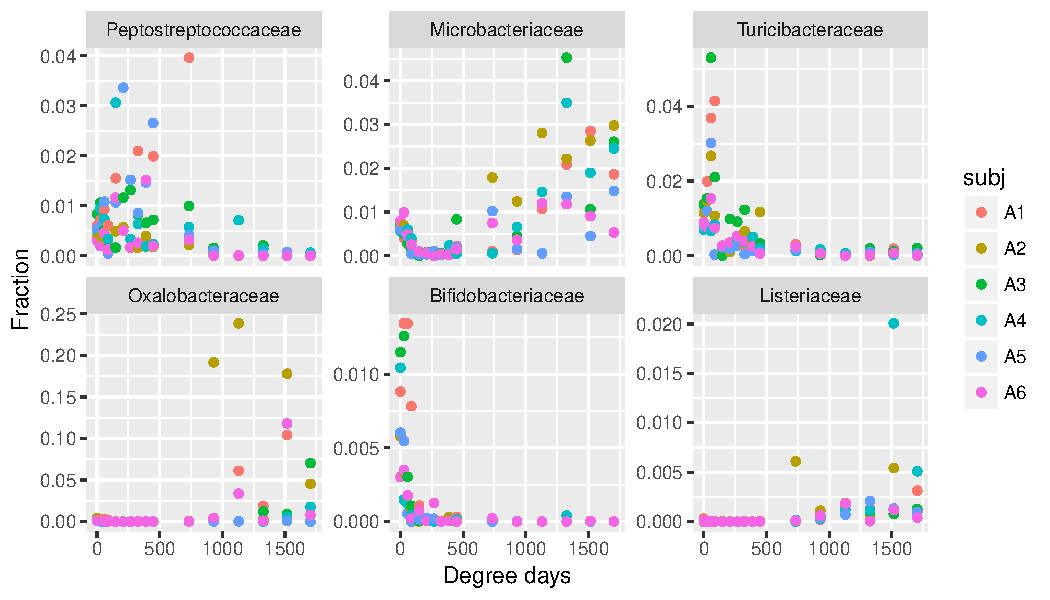
\includegraphics{../../only_families/all_time_steps/influential_family_taxa_panel}
  \caption{Some of the influential family-level taxa, by degree day}
  \label{fig:scatter_family_taxa}
\end{figure}

Figure \ref{fig:infl_family_taxa_stric_crit} shows the same type of
plot, but for the random forest model developed using the stricter
criterion.  Again, this criterion only allows taxa to be included if
the taxa makes up at least 1\% of the total counts for at least two
cadavers (can be on same or different days).  Therefore, this stricter
cutoff excludes Listeriaceae, and allows fewer (39) family-level taxa
to be included in the model.  Even so, the statistics presented in
Table \ref{tbl:family_all_data_model_stats} indicates that the
explanatory value of this model is almost as strong.

\begin{figure}
  \centering
  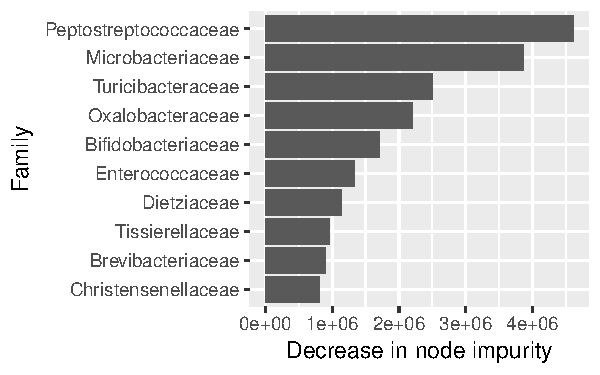
\includegraphics{../../only_families/all_time_steps/hit_1perc_twice/orig_units_all_data_families_barchart}
  \caption{Ten most influential family-level taxa, modeled using a stricter inclusion criterion}
  \label{fig:infl_family_taxa_stric_crit}
\end{figure}


\begin{table}
  \centering
\caption{\label{tbl:family_all_data_model_stats}Model statistics using family-level taxa}
\begin{tabular}{llll}
Inclusion cutoff & Units  & RMSE & Explained variation\\ \hline
1\% at least once (weaker)  & Orig.~units & 198.58 & 87.21\%\\
1\% at least twice (stricter) & Orig.~units & 207.18 & 86.08\% %%\\
%% 1\% at least once  & Sqrt.~units & 4.18 & 88.70\%\\
%% Didn't do the sqrt runs with the stricter cutoff.
\end{tabular}
\end{table}

To get an idea of the errors (also called residuals) made by the
random forest model, I used cross-validation runs.  Remember, the
cross-validations are done by randomly choosing 20\% of the dataset to
leave out the model-fitting procedure.  Then, the model (fitted on the
remaining 80\%) is used to estimate the responses for the observations
that were left out.  Figure \ref{fig:resids_cv_family_taxa}
illustrates the model errors (actual minus estimated) vs.~the actual
values, taken across 1000 cross-validation runs.  For the beginning of
the time period (lower degree days), the model is over-predicting,
while the opposite is true at the end of the time period.  The model
estimates are biased toward the average degree day.

\begin{figure}
  \centering
  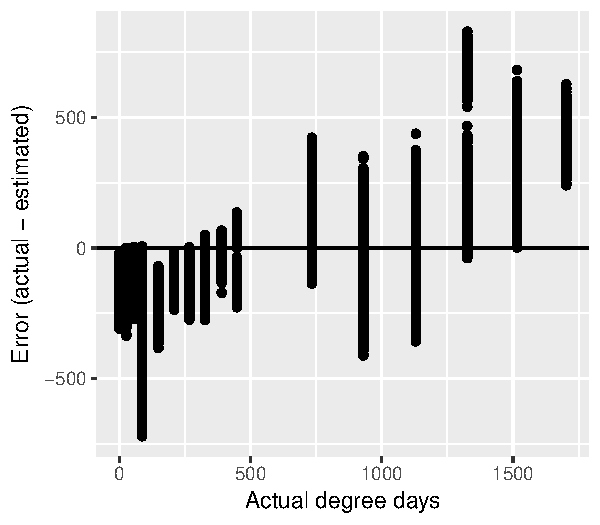
\includegraphics{../../only_families/all_time_steps/hit_1perc_twice/orig_units_all_data_families_residuals}
  \caption{Residuals from the cross-validation runs for the family taxa model}
  \label{fig:resids_cv_family_taxa}
\end{figure}

In practice, we would be using this model to predict the accumulated
degree days based on the counts of family-level taxa from a never
before observed cadaver.  The post mortem interval in such a case
would not necessarily correspond with a number of accumulated degree
days which we have observed before.  For instance, we might observe a
cadaver at a time associated with 100 degree days or 500 degree days.
To get a better idea about how the model might be expected to perform
in such a situation, we fit the model 96 times, leaving one subject
and one degree day out each time (16 degree days X 6 subjects).  Then,
we calculate the errors in the model estimates made for the subject
which was left out on the day which was left out.

Figure \ref{fig:leave_one_out_resids_family_taxa} shows the residuals
for all combinations of degree day and subject.  The RMSE for these
runs is about 274.8, which is higher than the RMSE for the model
including all data, which is given in Table
\ref{tbl:family_all_data_model_stats}.  This larger error stems from
two sources.  First, Table \ref{tbl:family_all_data_model_stats} shows
the model performance statistics based on fitting the model with all
available data, while these runs purposefully left out all the data
for a certain subject and for a certain day.  Second, by construction,
these test runs were conducted while omitting all information about a
particular degree day, so that there is a gap in the information
available.  In contrast, the RMSE associated with estimates for
left-out subjects on days that were not left out is only about 220.9

\begin{figure}
  \centering
  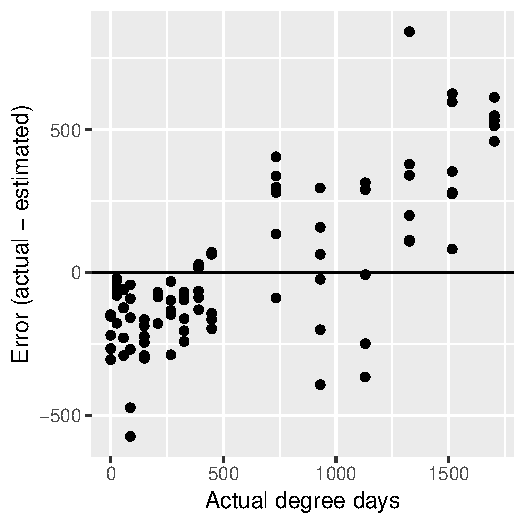
\includegraphics{../../only_families/all_time_steps/hit_1perc_twice/leave_out_one_subj_and_one_day_residuals}
  \caption{Residuals for model runs leaving out one subject and one day (family-level taxa)}
  \label{fig:leave_one_out_resids_family_taxa}
\end{figure}




\subsubsection{Results for order-level taxa}

For the order-level taxa, I also ran the analysis both ways, with the
stricter inclusion criterion (requiring 1\% for at least two cadavers)
and the weaker, original one.  Again, the model performance is similar
for both, so I think we should go with the stricter cutoff.  With the
stricter cutoff, the model considers 15 order-level taxa, versus 20
taxa with the original criterion.  The relevant performance statistics
are given in Table \ref{tbl:order_all_data_model_stats}.

\begin{table}
  \centering
  \caption{\label{tbl:order_all_data_model_stats}Model statistics using order-level taxa}
\begin{tabular}{llll}
Inclusion cutoff & Units  & RMSE & Explained variation\\ \hline
1\% at least once (weaker)  & Orig.~units & 230.19 & 82.81\%\\
1\% at least twice (stricter) & Orig.~units & 230.65 & 82.74\%
%% 1\% at least once  & Sqrt.~units &   4.38 & 87.62\%\\
%% Didn't do the sqrt runs with the stricter cutoff.
\end{tabular}
\end{table}

Figure \ref{fig:infl_order_taxa_stric_crit} shows the ten orders found
to be most influential in building the random forest model using the
stricter inclusion criterion.  These are similar to those found
previously, using the weaker inclusion criterion, with the one
noticeable difference being the elimination of the Bifidobacteriales
order.  This order exceeded 1\% of the total counts for only one
cadaver, so it could not be considered under the stricter inclusion
criterion.  Figure \ref{fig:scatter_order_taxa} shows the fraction of
counts associated with the six order taxa that were most influential
in the order-level random forest model.  Again, note the varying
scales of the y-axes across the panels.  The error patterns for the
models using order-level taxa are very similar to those for the
family-level taxa, so I haven't included them here.

\begin{figure}
  \centering
  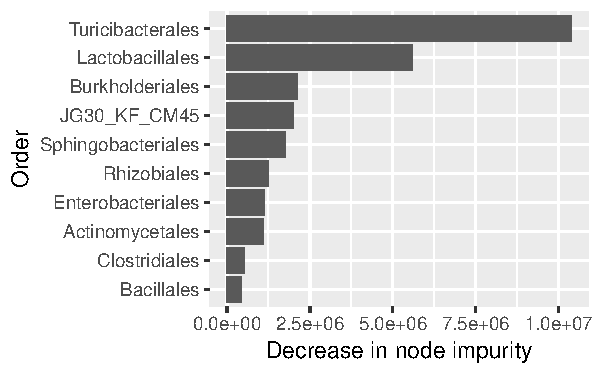
\includegraphics{../../only_orders/all_time_steps/hit_1perc_twice/orig_units_all_data_orders_barchart}
  \caption{Ten most influential order-level taxa, modeled using a stricter inclusion criterion}
  \label{fig:infl_order_taxa_stric_crit}
\end{figure}


\begin{figure}
  \centering
  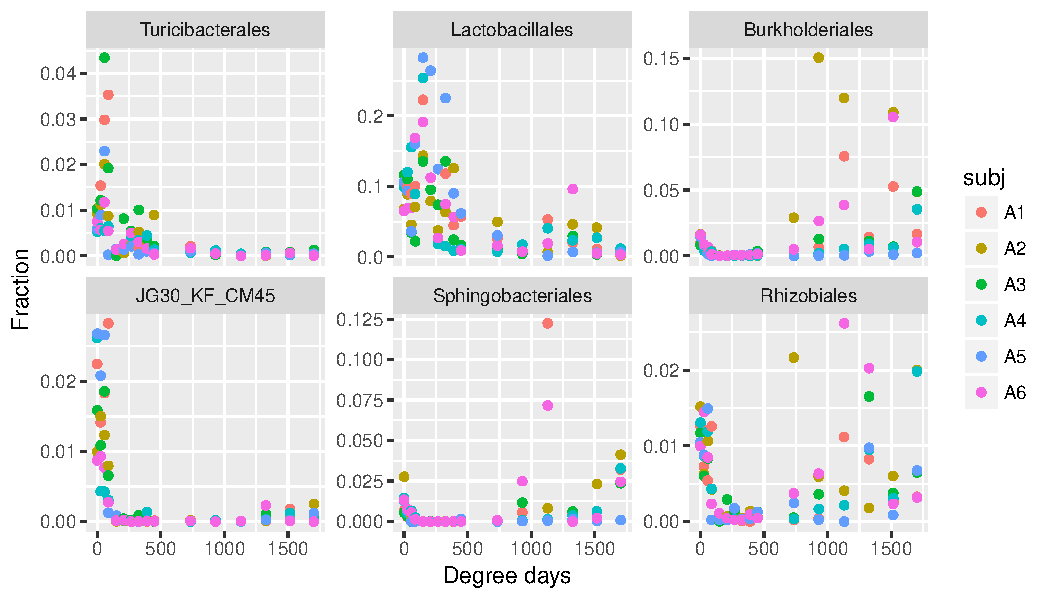
\includegraphics{../../only_orders/all_time_steps/influential_order_taxa_panel}
  \caption{Some of the influential order-level taxa, by degree day}
  \label{fig:scatter_order_taxa}
\end{figure}



\subsection{Models using only the first 15 days of data}

\subsubsection{Results for family-level taxa}

Table \ref{tbl:family_first_15days_model_stats} shows the model
performance statistics for the model using just the first 15 days of
family-level taxa.  Whether we use the weaker or stronger inclusion
criteria, model performance is much the same, so we go with the
stricter criterion for each of interpretation and implementation.  For
the first 15 days of data, we consider 35 possible family-level taxa.
As we might expect, the influential taxa for this early period are
different than those for the full time period.  The top 10 such taxa
are shown in Figure
\ref{fig:infl_family_taxa_first_15days_stric_crit}.  Scatterplots of
six of these taxa are found in Figure
\ref{fig:scatter_family_taxa_first_15days}.  Again, note the
difference in scaling of the y-axis among the various panels.

\begin{table}
  \centering
  \caption{\label{tbl:family_first_15days_model_stats}Model statistics using family-level taxa for the first 15 days}
\begin{tabular}{llll}
Inclusion cutoff & Units  & RMSE & Explained variation\\ \hline
1\% at least once (weaker) & Orig.~units & 64.98 & 81.99\%\\
1\% at least twice (stricter) & Orig.~units & 64.25 & 82.39\%
%% 1\% at least once  & Sqrt.~units & 2.31 & 87.87\%\\
%% 1\% at least twice & Sqrt.~units & 2.28 & 88.20\%
\end{tabular}
\end{table}

\begin{figure}
  \centering
  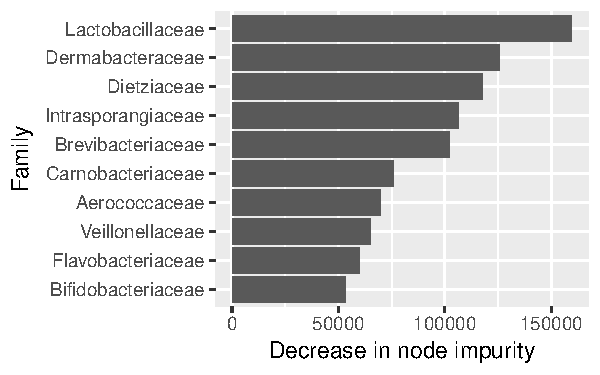
\includegraphics{../../only_families/first_two_weeks/hit_1perc_twice/orig_units_first_two_weeks_families_barchart}
  \caption{Ten most influential family-level taxa in the first 15 days, modeled using a stricter inclusion criterion}
  \label{fig:infl_family_taxa_first_15days_stric_crit}
\end{figure}

\begin{figure}
  \centering
  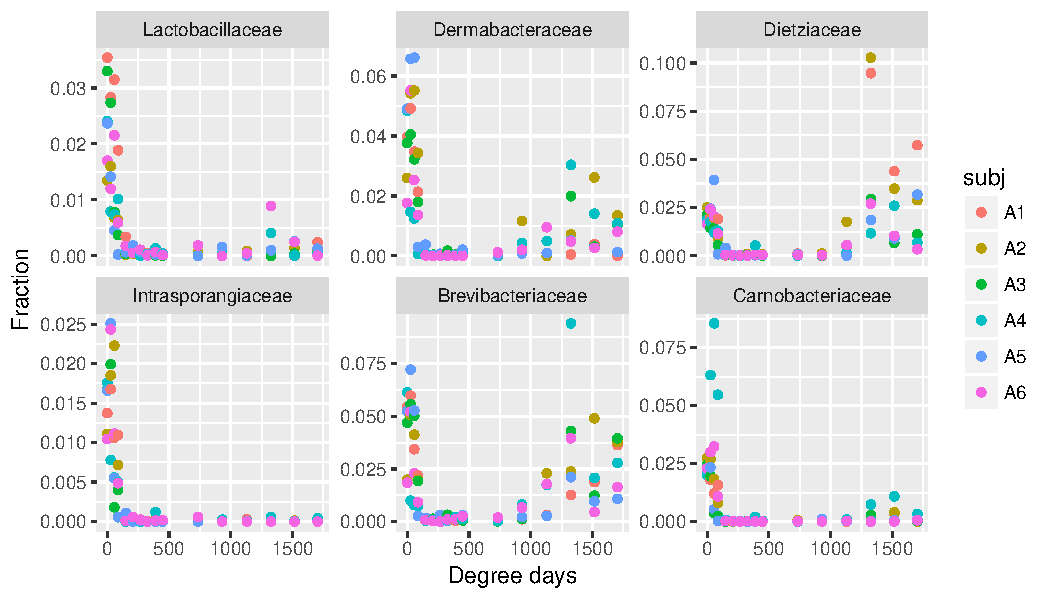
\includegraphics{../../only_families/first_two_weeks/influential_family_taxa_panel_first_two_weeks}
  \caption{Some of the influential family-level taxa, for the first 15 days}
  \label{fig:scatter_family_taxa_first_15days}
\end{figure}

Looking at the residuals, we see the same patterns that we saw for the
model using all time steps.  Figure
\ref{fig:resids_cv_first_15days_family_taxa} shows the errors
associated with 1000 cross-validation runs, with the training and
validation sets selected randomly.  However, since the analysis is
limited to the first two weeks, the RMSE is correspondingly lower.

\begin{figure}
  \centering
  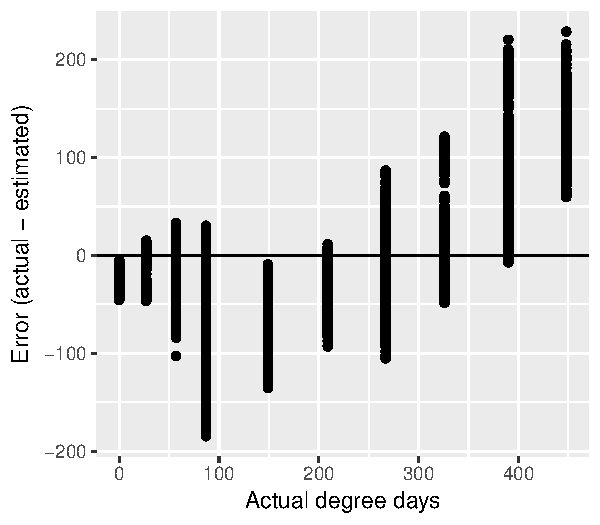
\includegraphics{../../only_families/first_two_weeks/hit_1perc_twice/orig_units_first_two_weeks_families_residuals}
  \caption{Residuals from the cross-validation runs for the family taxa model, first 15 days}
  \label{fig:resids_cv_first_15days_family_taxa}
\end{figure}

Figure \ref{fig:leave_out_one_resids_family_taxa_first_15days} shows
the residuals when we each combination of one subject and one time
step out of the model-fitting process.  Again, this is very similar to
the pattern we saw when using the data from the whole time period.
The RMSE for these runs is about 83.5.  This means that in a real-life
situation, in which it's likely that we do not have observations from
the applicable degree day, the RMSE is substantially higher than the
RMSE for the fitted model.
%% The RMSE for situations where we are predicting the left-out
%% individual for days which are present in the model is about 66.1.

\begin{figure}
  \centering
  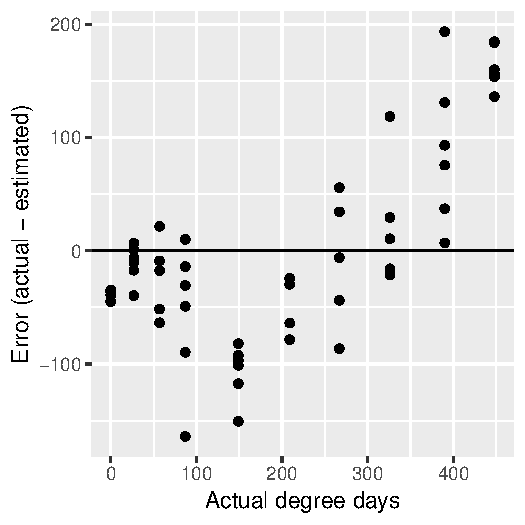
\includegraphics{../../only_families/first_two_weeks/hit_1perc_twice/leave_out_one_subj_and_one_day_residuals}
  \caption{Residuals for model runs leaving out one subject and one day, first 15 days (family-level taxa)}
  \label{fig:leave_out_one_resids_family_taxa_first_15days}
\end{figure}


\subsubsection{Results for order-level taxa}

Looking at the model for the first 15 days, using the order-level
taxa, the models with the stricter and weaker inclusion cutoffs are
again very similar.  The model performance statistics are shown in the
Table \ref{tbl:order_first_15days_model_stats}.  We stick with the
stricter inclusion criterion, which utilizes 14 orders in the random
forest model.  Figure
\ref{fig:infl_order_taxa_first_15days_stric_crit} shows the 10 most
influential order-level taxa in the model, and Figure
\ref{fig:scatter_order_taxa_first_15days} provides a sense of how the
fractions attributable to six of these taxa are changing over the
first 15 days.

\begin{table}
  \centering
  \caption{\label{tbl:order_first_15days_model_stats}Model statistics using order-level taxa for the first 15 days}
\begin{tabular}{llll}
Inclusion cutoff & Units  & RMSE & Explained variation\\ \hline
1\% at least once (weaker) & Orig.~units & 53.93 & 87.59\%\\
1\% at least twice (stricter) & Orig.~units & 54.68 & 87.25\%
%% 1\% at least once  & Sqrt.~units & 2.01 & 90.81\%
%% 1\% at least twice & Sqrt.~units & 2.02 & 90.68\%
\end{tabular}
\end{table}

\begin{figure}
  \centering
  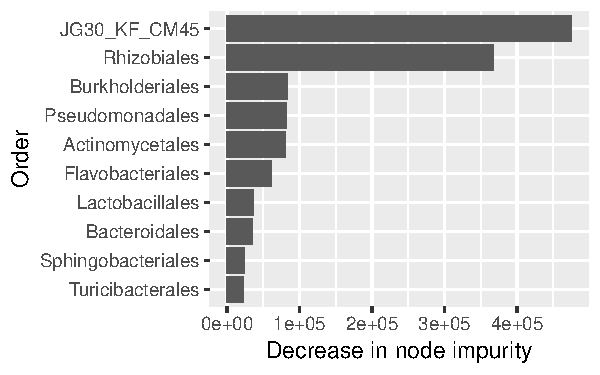
\includegraphics{../../only_orders/first_two_weeks/hit_1perc_twice/orig_units_first_two_weeks_orders_barchart}
  \caption{Ten most influential order-level taxa in the first 15 days, modeled using a stricter inclusion criterion}
  \label{fig:infl_order_taxa_first_15days_stric_crit}
\end{figure}

\begin{figure}
  \centering
  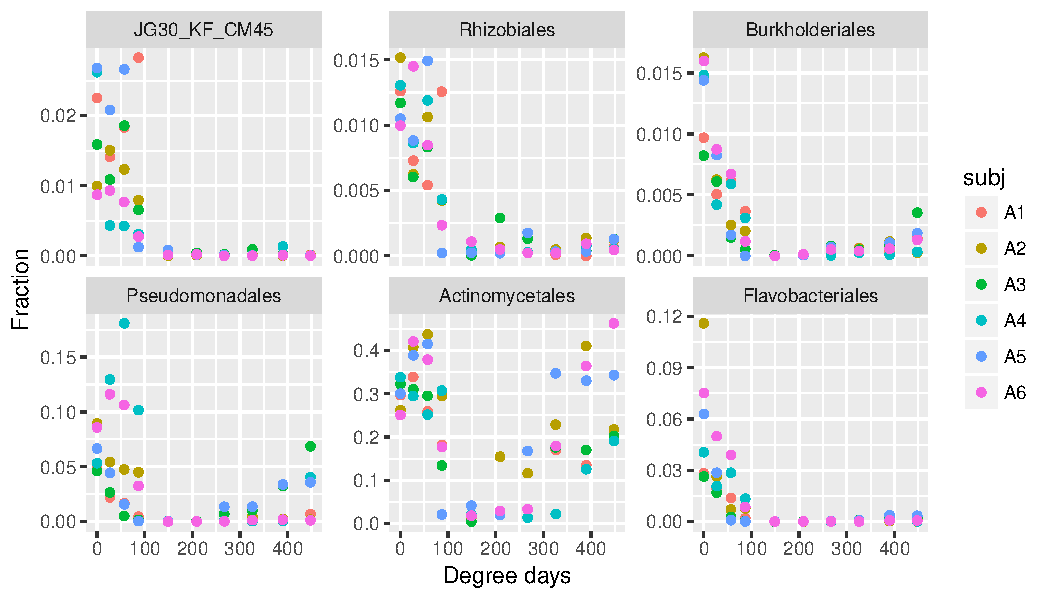
\includegraphics{../../only_orders/first_two_weeks/influential_order_taxa_panel_first_two_weeks}
  \caption{Some of the influential order-level taxa, for the first 15 days}
  \label{fig:scatter_order_taxa_first_15days}
\end{figure}


\section{Working with Luisa's eukaryote data}

\subsection{Overview}

I applied the same methods to Luisa's eukaryote data, again focusing
on family-level and order-level taxa.  I did not find any day/subject
combination with an unusually low count, as I did for subject A3 on
day 40 of Shane's data.  However, I did find very small numbers of
counts from orders Mammalia and Aves, which I excluded from the
analysis.

The cross-validation procedures I used were also the same as those
used previously.  I focused on the stricter inclusion criterion,
meaning that, for inclusion in the analysis, a taxon must make up more
than 1\% of the total daily counts on at least 2 cadavers.  Again,
this reduces the number of taxa to consider, and hopefully makes the
analysis more resistant to outliers and easier to implement in a
real-life estimation.

\subsection{All time steps}

\subsubsection{Results for family-level taxa}

The model statistics for the final random forest model, using both the
weaker and stronger inclusion criteria, are found in Table
\ref{tbl:eukaryote_family_all_data_model_stats}.  As before, the
goodness-of-fit is very similar, so for the remainder of the analyses,
I will stick with models following the stricter criterion.  Note that
this model seems to fit better than the model making use of the
previous bacteria-only dataset.

\begin{table}
  \centering
\caption{\label{tbl:eukaryote_family_all_data_model_stats}Model statistics using family-level eukaryote taxa}
\begin{tabular}{llll}
Inclusion cutoff & Units  & RMSE & Explained variation\\ \hline
1\% at least once (weaker)  & Orig.~units & 175.7 & 89.80\%\\
1\% at least twice (stricter) & Orig.~units & 178.1 & 89.51\% 
\end{tabular}
\end{table}

Thirty-nine taxa were considered in the random forest model, using the
stricter criterion.  The top 10 taxa indicated by the model to be the
most influential in the random forest model are shown in Figure
\ref{fig:infl_eukaryote_family_taxa}.  A scatterplot of
fractional make-up vs. degree day is shown for several of these taxa
in Figure \ref{fig:scatter_eukaryote_family_taxa}.

\begin{figure}
  \centering
  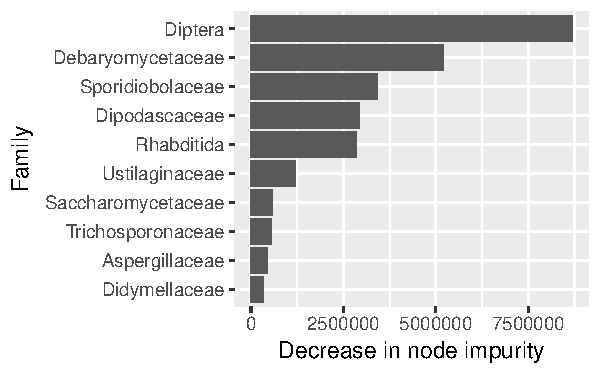
\includegraphics{../../../eukaryote_data/only_families/all_time_steps/hit_1perc_twice/orig_units_all_data_families_barchart}
  \caption{Ten most influential eukaryote family-level taxa}
  \label{fig:infl_eukaryote_family_taxa}
\end{figure}

\begin{figure}
  \centering
  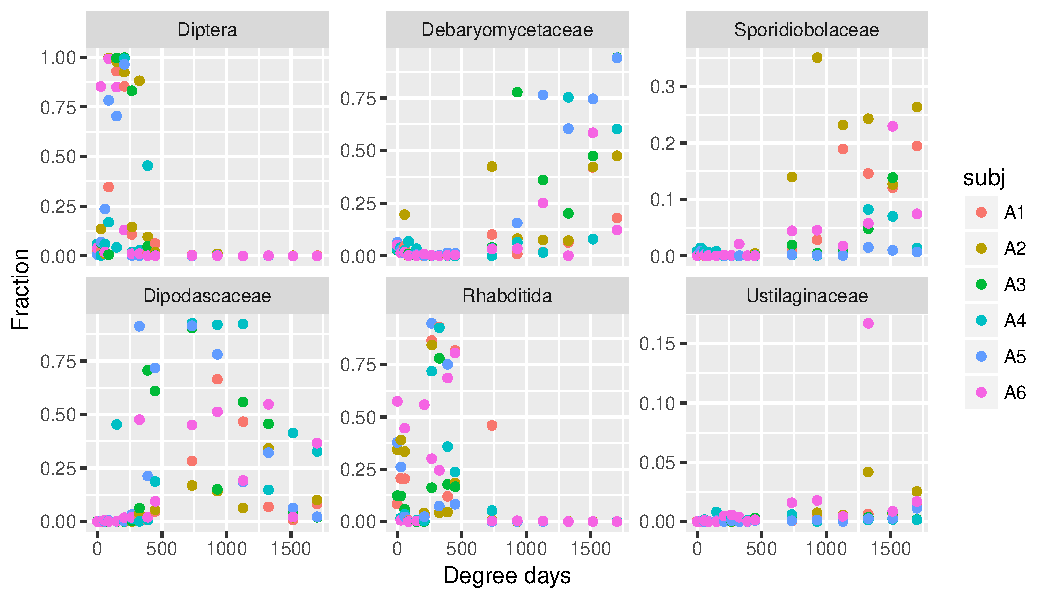
\includegraphics{../../../eukaryote_data/only_families/all_time_steps/influential_family_taxa_panel}
  \caption{Some of the influential eukaryote family-level taxa, by degree day}
  \label{fig:scatter_eukaryote_family_taxa}
\end{figure}

Figure \ref{fig:resids_cv_eukaryote_family_taxa} shows a scatterplot
of the errors vs.~the actual degree days, across all 1000
cross-validation runs.  The pattern is much the same as those
identified in the earlier sections, using Shane's data.  In a
real-world application, though, we may not have any observations
corresponding to the actual degree days accumulated post mortem.
Figure \ref{fig:leave_one_out_resids_eukaryote_family_taxa} shows
these residuals, which again show patterns similar to those seen in
earlier sections.  The root mean squared estimation error in these
cases is about 243.6, which is better than that using the
bacteria-only dataset.
%% The RMSE for predictions of left-out individuals on days where we do
%% have data is about 186.2.

\begin{figure}
  \centering
  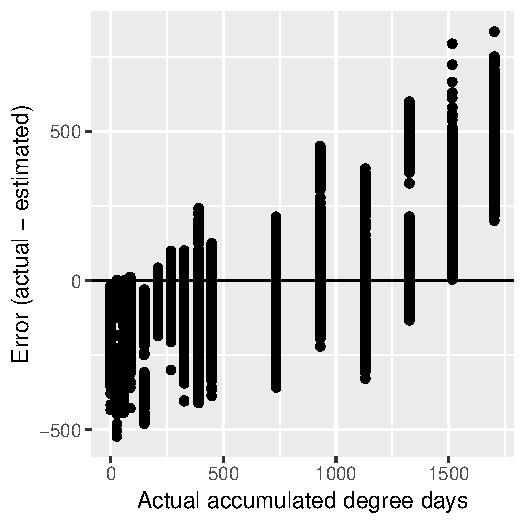
\includegraphics{../../../eukaryote_data/only_families/all_time_steps/hit_1perc_twice/orig_units_all_data_families_residuals}
  \caption{Residuals from the cross-validation runs for the eukaryote family-level taxa model}
  \label{fig:resids_cv_eukaryote_family_taxa}
\end{figure}

\begin{figure}
  \centering
  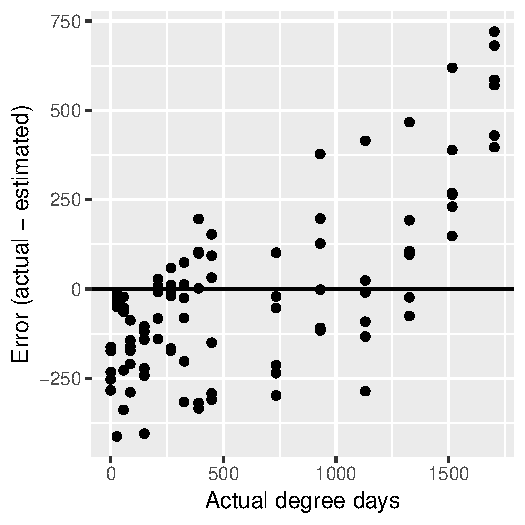
\includegraphics{../../../eukaryote_data/only_families/all_time_steps/hit_1perc_twice/leave_out_one_subj_and_one_day_residuals}
  \caption{Residuals for model runs leaving out one subject and one day (eukaryote family-level taxa)}
  \label{fig:leave_one_out_resids_eukaryote_family_taxa}
\end{figure}


\subsubsection{Results for order-level taxa}

Table \ref{tbl:eukaryote_order_all_data_model_stats} shows the model
performance statistics for the eukaryote order-level taxa, which again
seems to indicated a better fit than the model for the same level taxa
in Shane's dataset.  Figures \ref{fig:infl_eukaryote_order_taxa} and
\ref{fig:scatter_eukaryote_order_taxa} show some of the influential
order-level taxa.

\begin{table}
  \centering
\caption{\label{tbl:eukaryote_order_all_data_model_stats}Model statistics using order-level eukaryote taxa}
\begin{tabular}{llll}
Inclusion cutoff & Units  & RMSE & Explained variation\\ \hline
1\% at least twice (stricter) & Orig.~units & 193.2 & 87.67\% 
\end{tabular}
\end{table}

\begin{figure}
  \centering
  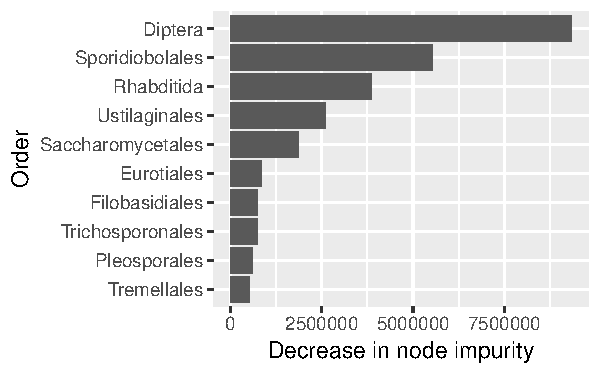
\includegraphics{../../../eukaryote_data/only_orders/all_time_steps/hit_1perc_twice/orig_units_all_data_orders_barchart}
  \caption{Ten most influential eukaryote order-level taxa}
  \label{fig:infl_eukaryote_order_taxa}
\end{figure}

\begin{figure}
  \centering
  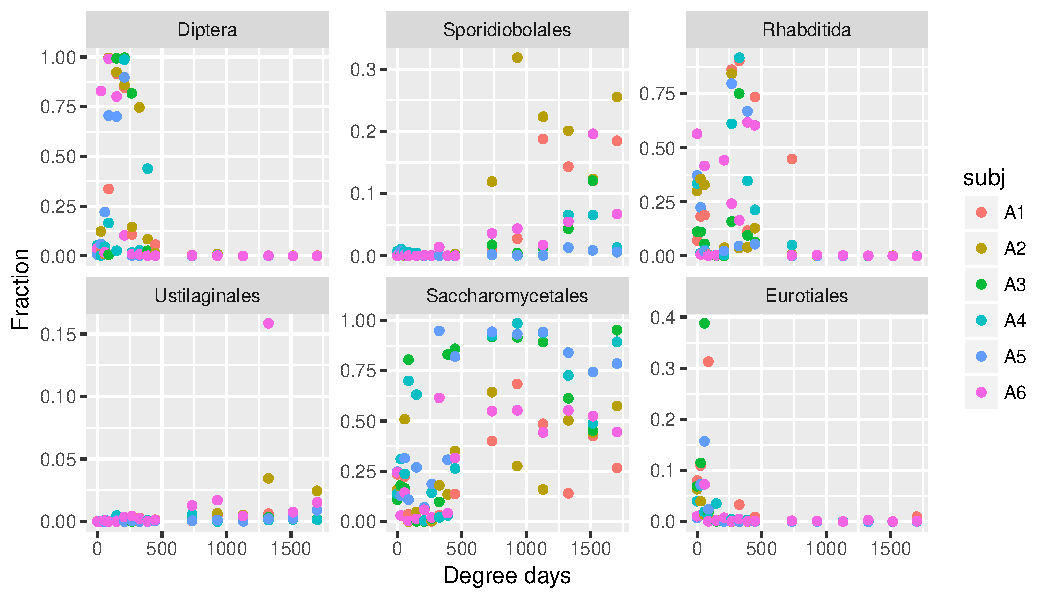
\includegraphics{../../../eukaryote_data/only_orders/all_time_steps/influential_order_taxa_panel}
  \caption{Some of the influential eukaryote order-level taxa, by degree day}
  \label{fig:scatter_eukaryote_order_taxa}
\end{figure}


\end{document}

